\begin{problem}{피자 배틀}{표준 입력(stdin)}{표준 출력(stdout)}{5\,초}{1024\,MB}

실버는 피자를 매우 빠르게 먹는다. 실버의 속도에 대적할 수 있는 유일한 상대는 그의 동생 브론즈이다. 두 사람의 피자 먹는 속도는 초당 $1$단위로 동일하다.

실버와 브론즈는 서로의 능력을 과시하기 위해 게임을 하기로 했다. 게임은 $N$개의 조각으로 이루어진 원형의 피자에서 진행되며, 각각의 조각의 크기는 $1$ 이상 $100$ 이하의 정수다. 두 사람의 목표는 피자를 최대한 많이 먹는 것이다.

실버부터 시작하여 피자 조각을 고르는데, 첫 번째 조각은 아무렇게나 골라도 되지만, 그 다음 조각부터는 바깥쪽에 있는 조각만을 골라야 한다. 즉, 고르려고 하는 조각의 양 옆 중 한 곳 이상이 비어 있어야 한다.

처음에 실버가 피자 조각을 고른 뒤 $0.5$초 후에 브론즈가 피자 조각을 고른다. 또한, 두 플레이어는 선택한 피자 조각을 다 먹은 직후에 다음 피자 조각을 골라야 한다. 이 때 각자가 피자 조각을 고르는 시간은 무시한다.

피자의 크기가 순서대로 $1$, $2$, $3$, $4$일 때 가능한 게임 양상의 예시는 다음과 같다.
\begin{itemize}
    \item[$t=0$:] 실버가 $3$을 고르고 먹기 시작함.
    \item[$t=0.5$:] 브론즈는 $2$와 $4$ 중 하나를 골라서 먹을 수 있음. $2$를 고르고 먹기 시작함.
    \item[$t=2.5$:] 브론즈가 $2$짜리 조각을 다 먹음. $1$과 $4$ 중 $1$을 골라서 먹기 시작.
    \item[$t=3$:] 실버가 $3$짜리 조각을 다 먹음. $4$를 골라서 먹기 시작.
    \item[$t=3.5$:] 브론즈가 $1$짜리 조각을 다 먹었지만, 고를 피자 조각이 없으므로 더 이상 피자를 못 먹음.
    \item[$t=7$:] 실버가 $4$짜리 조각을 다 먹음.
\end{itemize}

최종 결과: 실버 $7$, 브론즈 $3$

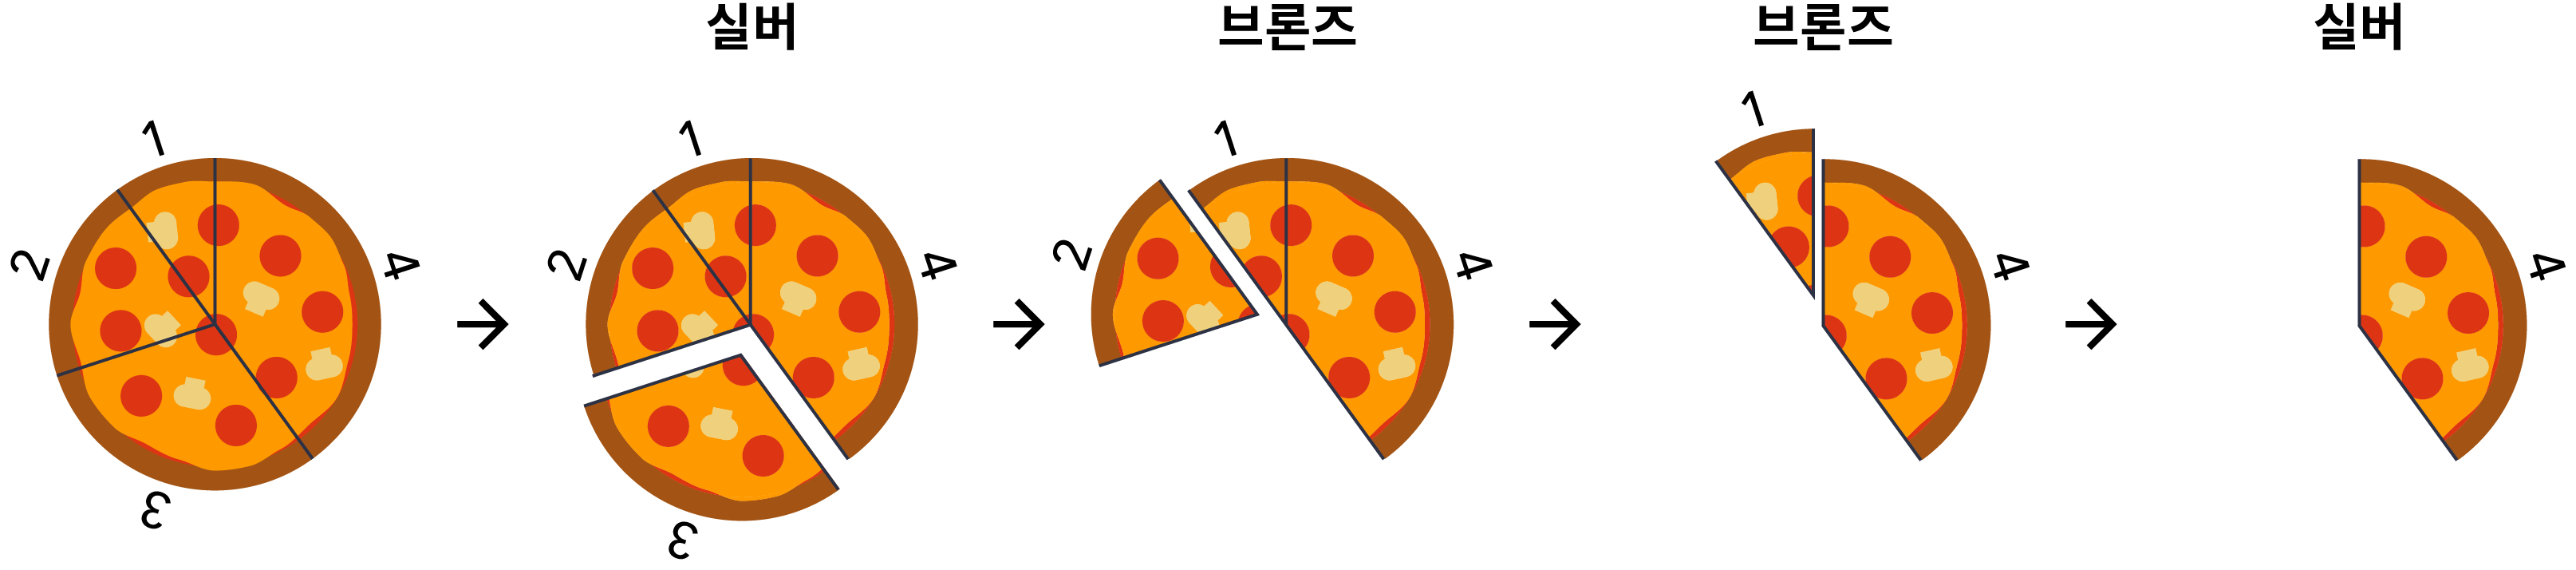
\includegraphics[width=\textwidth]{UCPC 2020/problems/pizza-battle/picture/pizza1.png}
\begin{center}
    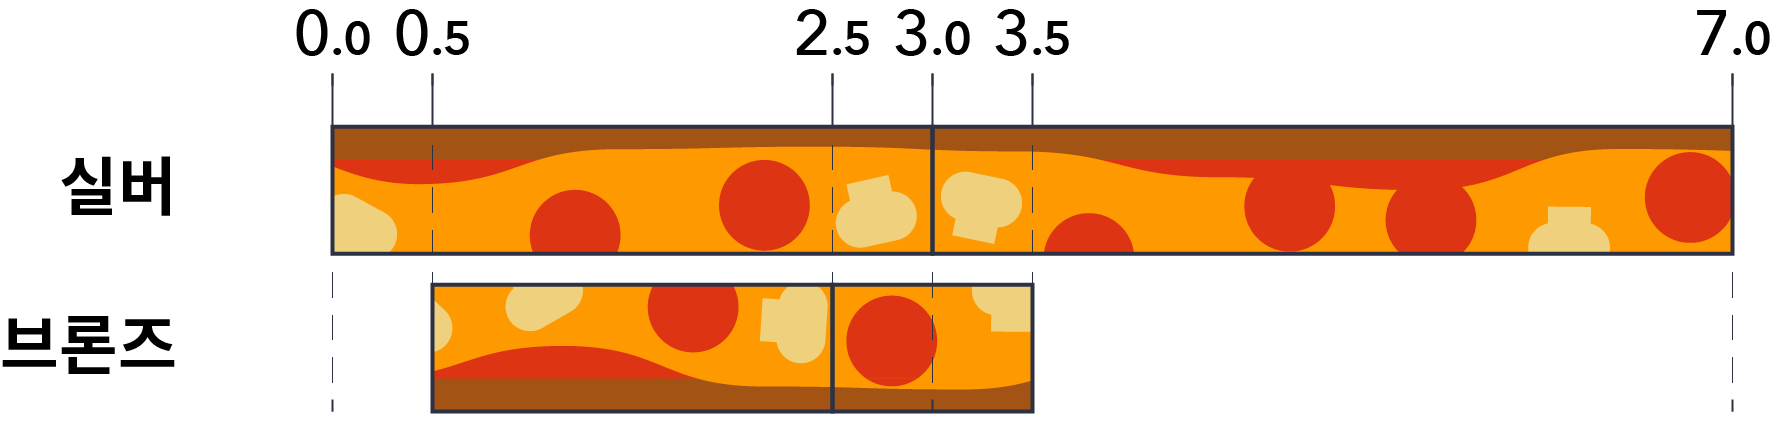
\includegraphics[width=.5\textwidth]{UCPC 2020/problems/pizza-battle/picture/pizza2.png}
\end{center}

예시에 있는 두 사람의 플레이는 최선의 플레이가 아닐 수 있음에 유의한다. 피자가 주어지면, 두 사람이 최선의 전략으로 플레이했을 때 실버가 먹게 되는 피자의 양을 구하는 프로그램을 작성하여라.

\InputFile
첫 번째 줄에 피자 조각의 수 $N$이 주어진다. $(1 \leq N \leq 1\ 000)$

두 번째 줄에 $N$개의 피자 조각의 크기가 시계 방향 순서대로 주어진다. 피자 조각의 크기는 $1$ 이상 $100$ 이하의 정수다. 원형이므로 $1$번 피자 조각과 $N$번 피자 조각은 연결되어 있다.

\OutputFile
두 사람이 최선의 전략으로 플레이했을 때 실버가 먹게 되는 피자의 양을 출력한다.

\Examples

\begin{example}
\exmp{
4
1 2 3 4
}{%
5
}%
\exmp{
4
1 3 2 4
}{%
6
}%
\end{example}

\end{problem}

